\section{The Isotropic ZGV Ring}

\subsection{Exact Rayleigh--Lamb reference}

We restrict the isotropic reference calculation to the selected symmetric
$S_1$ branch and the configured local window around its zero-group-velocity
(ZGV) state.  Within that scope, the traction-free Rayleigh--Lamb determinant
is desingularized before root finding, so a vanishing shear thickness
wavenumber cannot be mistaken for a physical root.  With
$\kappa=kh$ and $\Omega=\omega h/c_T$, simultaneously solving
$D_S=D_{S,k}=0$ gives the dimensionless location
$\kappa_0=\ZGVKappa$ and frequency $\Omega_0=\ZGVOmega$; implicit
differentiation gives the positive dimensionless radial curvature
$a=\mathrm d^2\Omega/\mathrm d\kappa^2=\ZGVCurvature$.  These quantities
characterize one simple local branch,
not all symmetric, antisymmetric, or shear-horizontal branches of the plate.

The reference starts from the physical face-traction matrix rather than a
quotient form of the classical dispersion relation
\citep{lamb1917waves}.  Rescaling the shear potential produces the regular
determinant in Eq.~\eqref{eq:desingularized-determinant}, which remains finite
through the shear cutoff.  The nonzero frequency derivative then identifies a
smooth scalar branch, while Eqs.~\eqref{eq:implicit-first-derivative} and
\eqref{eq:zgv-curvature} convert the double condition on $D_S$ into zero radial
group velocity and a directly differentiated curvature.  The independently
refined values declared in Eq.~\eqref{eq:reference-isotropic-zgv-values}
therefore come from the exact isotropic determinant and are not fitted to the
subsequent spectral calculation.

Near the critical radius, the branch is described by
$\Omega=\Omega_0+a(\kappa-\kappa_0)^2/2$ to leading order.  The positive sign
of $a$ makes the selected state a radial minimum, consistent with the familiar
local ZGV geometry and its established role in long-lived plate responses
\citep{prada2008power}.  This local quadratic statement is used only inside
the configured window; it does not replace the exact branch away from the
reference point.

\subsection{Morse--Bott geometry}

% Claim C1
Within a sufficiently thin local annulus on the selected isotropic branch,
rotational invariance lifts the radial ZGV state to the critical ring
$\Gamma_0=\{\boldsymbol\kappa\in\mathbb{R}^2:
\abs{\boldsymbol\kappa}=\kappa_0\}$, where
\(\boldsymbol\kappa=h\mathbf k^{\mathrm{phys}}\).  We use the
Morse--Bott classification to state its degeneracy precisely: the radial
normal direction is nondegenerate, whereas the tangential zero direction is
enforced by continuous rotational symmetry.  This is a plate-specific
classification of the familiar isotropic ZGV circle, not an assertion that
the circle itself is newly found, and it requires the local branch to remain
simple and uniformly separated from neighbouring modes.

The Cartesian Hessian with respect to \(\boldsymbol\kappa\) on the ring is
$a\,\mathbf e_r\mathbf e_r^{\mathsf T}$, with spectrum $\{a,0\}$, as shown in
Eq.~\eqref{eq:zgv-ring-hessian}.  Its kernel is therefore exactly the tangent
space of $\Gamma_0$, while its restriction to the radial normal space is the
nonsingular scalar form $[a]$ in
Eq.~\eqref{eq:morse-bott-kernel-and-normal-form}.  These two facts meet the
normal-nondegeneracy condition of Theorem~\ref{thm:morse-bott-ring}
\citep{bott1954critical}.  They also distinguish one connected critical
manifold from a collection of unrelated isolated points.  Cases with zero
radial curvature or a closing eigengap lie outside the theorem.

Figure~\ref{fig:geometry-mechanism} summarizes the resulting geometry and
previews its weak-cubic unfolding.  The isotropic contours share a stationary
circle, whereas the anisotropic panel places the refined full-wave minima and
saddles inside the declared local annulus.  Their count and classification
are justified with the full anisotropic calculation below; only the final
dimension-and-decay map is conceptual.
Related anisotropic ZGV organization and temporal interference have already
been reported \citep{kiefer2023beating}; here the diagram serves only as a
roadmap to the coefficient-resolved calculation.

\begin{figure}
  \centering
  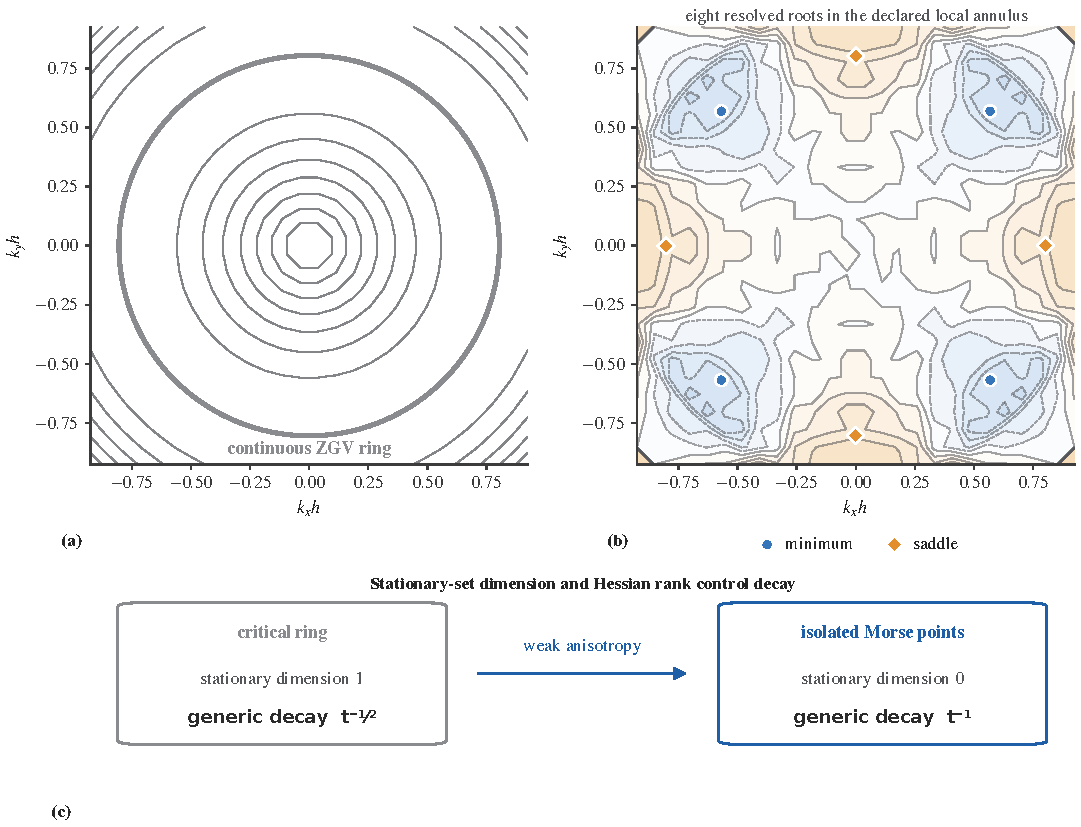
\includegraphics[width=\textwidth]{../figures/main/figure_01_geometry_mechanism.pdf}
  \caption{\FigureOneCaption}
  \label{fig:geometry-mechanism}
\end{figure}

\subsection{Independent spectral verification}

We next test the exact reference with an independent thickness-resolved
calculation, restricted to the same configured local window and tracked
spectral branch.  The generalized Hermitian eigenproblem uses traction-free
natural boundary conditions and no Rayleigh--Lamb determinant.  Thus its
agreement with the exact root checks a distinct numerical representation of
the elastic field.  This is a computation-only verification rather than an
experiment: no measured resonance, fitted material parameter, or laboratory
observable enters the comparison.

The spectral weak form of Eq.~\eqref{eq:spectral-weak-form} resolves all
displacement components through the thickness.  Branch continuity is enforced
by the mass-weighted overlap procedure in Algorithm~\ref{alg:mode-tracking},
and queries are rejected when the local separation condition in
Eq.~\eqref{eq:eigengap-rejection} is not met.  Across the declared order
sweep, the normalized eigen-residual of
Eq.~\eqref{eq:normalized-eigen-residual}, the mass-orthogonality defect of
Eq.~\eqref{eq:mass-orthogonality-defect}, and the exact-reference errors remain
small while the relative eigengap stays
open.  This simultaneously checks branch identity, field resolution, and the
simple-eigenvalue hypothesis used by Theorem~\ref{thm:morse-bott-ring}; it is
not a claim about branches outside the tracked window.  Spectral guided-wave
discretization itself is established methodology \citep{adamou2004spectral}.

Figure~\ref{fig:isotropic-zgv} separates the four pieces of this check.  The
tracked symmetric branch has a local minimum at the computed
$(\ZGVKappa,\ZGVOmega)$ reference; the exact branch and its quadratic form
with curvature $\ZGVCurvature$ agree over the declared local comparison
interval.  The convergence panel reports errors and eigengap
together, preventing apparent frequency agreement from masking branch
coalescence.  Finally, the mass-normalized mode panel shows the
through-thickness component magnitudes and their squared-displacement proxy;
because it plots magnitudes, it is not used as a signed parity test.  These mutually
consistent diagnostics support
the Morse--Bott statement only for the selected uniformly gapped local branch.

\begin{figure}
  \centering
  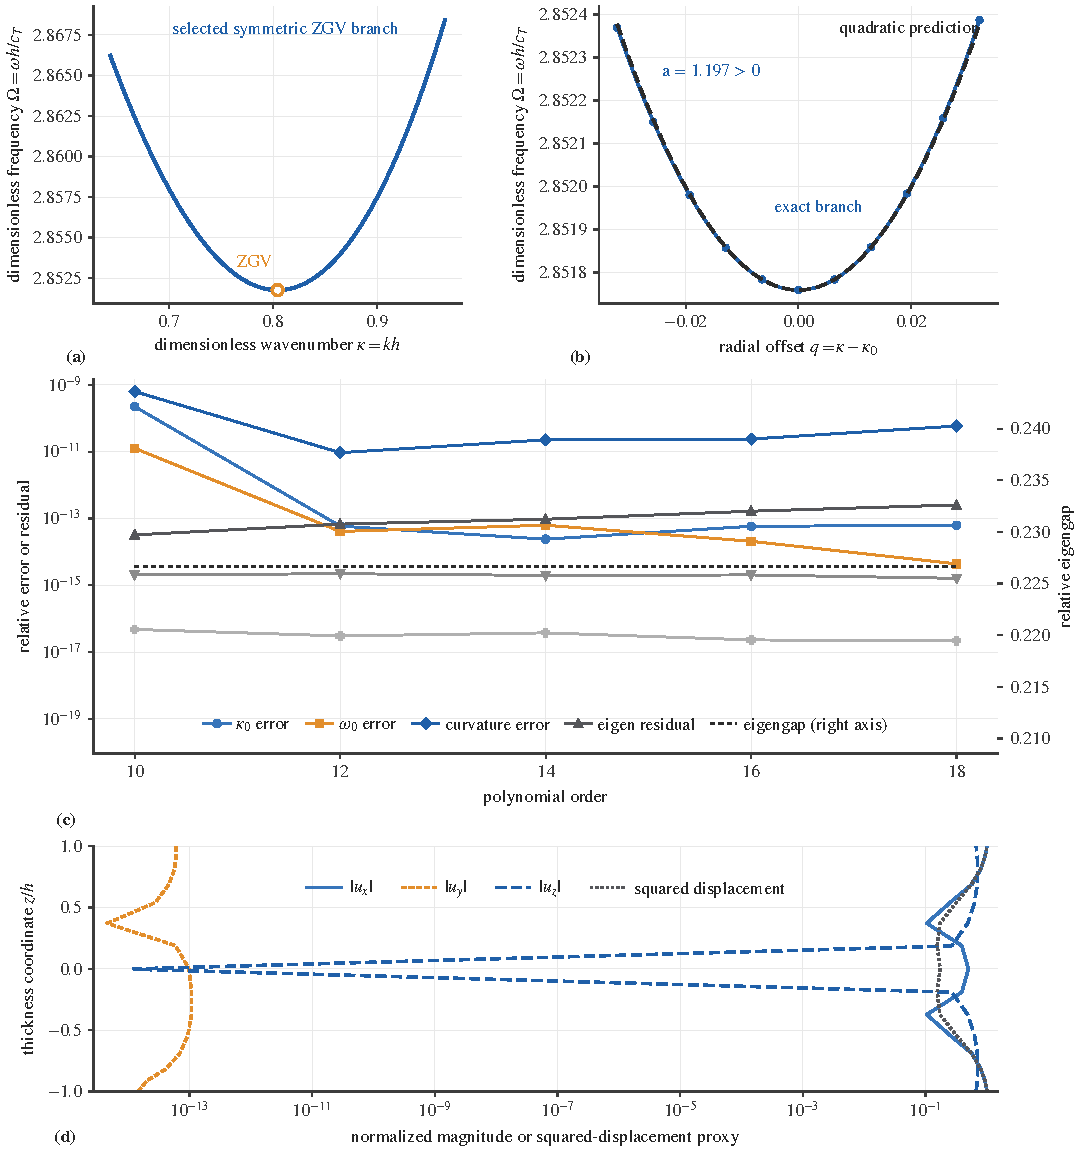
\includegraphics[width=\textwidth]{../figures/main/figure_02_isotropic_zgv.pdf}
  \caption{\FigureTwoCaption}
  \label{fig:isotropic-zgv}
\end{figure}
